\chapter{Overview of the triangulation method}
\label{chap:LOST}

In the previous chapter, the ESKF was introduced as a method capable of updating the state using camera measurements, provided by the precise localization coordinates of visible feature points are known. However, in practical applications, assuming prior knowledge of the positions of these visible feature points is often untenable. Consequently, there arises the need to estimate these vectors, a process commonly referred to as triangulation.

This chapter provides an in-depth look at the triangulation method applied in this study, with a focus on its integration into the visual-inertial navigation system. The foundation of this method draws from \cite{absolute-triangulation}, utilizing the core equations as described therein. However, their approach only takes into account uncertainties in the camera measurements, but the current system requires consideration of uncertainties in the states too.

The central objective of this chapter is to explain the key components and modifications in the custom-made triangulation approach. In particular, answers will be given to questions such as how position and orientation are involved in the LOST equations, and how can be formed the recursive version of LOST.

\section{Problem statement}

The modern triangulation problem takes on one of two forms: intersection or resection \cite{ResectionInSurvey_1918}, shown in the figure \ref{fig:intersec-resec}.

\begin{figure}[!ht]
    \centering
    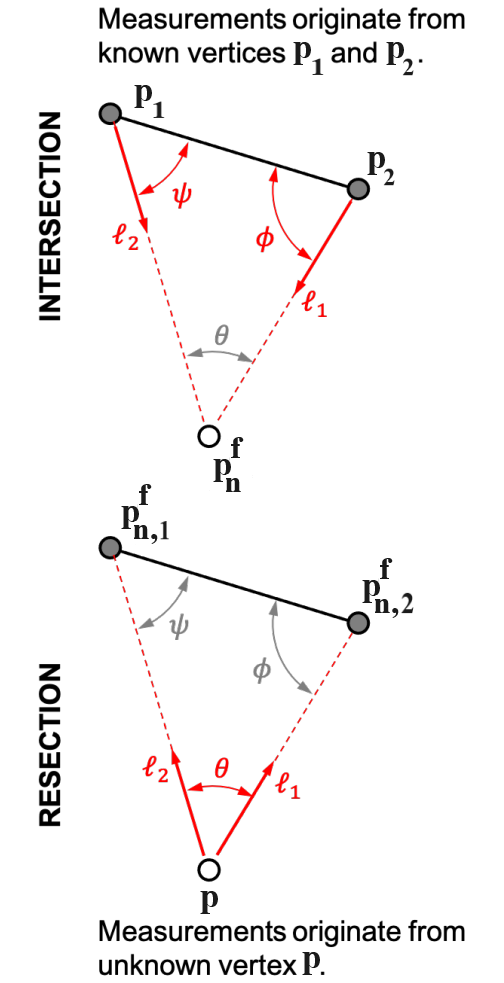
\includegraphics[width=0.35\textwidth]{figures/intersec-resec.png}
    \caption{Illustration of intersection (top) and resection (bottom) forms of the triangulation problem (\cite{absolute-triangulation}: page 3)}
    \label{fig:intersec-resec}
\end{figure}

The main difference between the two formalizations is that the intersection assumes measurements taken from known vertices ($\mathbf{p}_1$, $\mathbf{p}_2$). These vertices express the camera positions at each measurement in the NED frame ($\mathbf{p}_n^c$) and the goal is to determine the position of a visible feature point ($\mathbf{p}_n^f$). On the other hand, the resection problem supposes known visible vertices ($\mathbf{p}_{n, 1}^f$, $\mathbf{p}_{n, 2}^f$) and aims to estimate the position where the measurement was taken ($\mathbf{p}$).

The intersection problem has many practical applications such as satellite orbit determination \cite{TriagulationSpaceOrb1, TriagulationSpaceOrb2}, and 3-D scene reconstruction usually called Structure from Motion (SfM) \cite{Triang3D1, Triang3D2, Triang3D3}. The resection problem describes the vehicle localization problem that is generally included in navigation applications \cite{rel-nav-1, rel-nav-2, TriangNav}. In this project, both forms are applied, because LOST is used to optimize 3-D coordinates of visible feature points which means a 3-D reconstruction of the environment. On the contrary, the Kalman filter update is the form of a resection problem in the sense that the optimized LOST estimates are used to improve the state estimates.

\subsection{Line of sight (LOS) measurements}

The triangulation problem typically involves angles acquired through various optical instruments. In vehicle navigation, angles are often derived from images captured by cameras or telescopes. Regardless of the specific application, the angle measurements obtained through these optical instruments describe the direction from the sensor to the observed point. In other words, they express the path from one vertex of a triangle to another, and this direction represents a straight line connecting these two points, commonly known as the "line of sight" (LOS).

Before I delve into the details, it's important to establish a few mathematical notation:
\begin{itemize}
    \item The actual measurement is $\begin{bmatrix} u_i & v_i & f\end{bmatrix}^T = \overline{\mathbf{u}}_i = \mathbf{K}\mathbf{u}_i$, but the LOST algorithm uses LOS measurement ($\mathbf{u}$, Figure \ref{fig:camera-system}) that can be derived from actual measurement as $\mathbf{u}_i=\mathbf{K}^{-1}\overline{\mathbf{u}}_i$. However, it is important to emphasize that this transformation accounts for both the adjustment of the principal point and multiplying the vector with the focal length. Later merely introduces a scaling factor, which is inherently resolved in LOST equations, therefore it is enough to compensate the principal point.
    \item The feature's position ($\mathbf{p}_c^f$) and the LOS measurement differ only with a scaling factor: $\mathbf{u}_i \propto \mathbf{a}_i \propto \mathbf{p}_{c,i}^f$, where $\mathbf{a}_i=\frac{\mathbf{u}_i}{||\mathbf{u}_i||} = \frac{\mathbf{p_{c,i}^f}}{||\mathbf{p}_{c,i}^f||}$ 
    \item $\mathbf{p}_{c,i}^f=\rho\mathbf{a}_i$, where $\rho$ denotes the range from the camera center to the observed point
\end{itemize}

\section{LOST method}

When more than 2 LOS measurements are available the polynomial methods do not scale well \cite{absolute-triangulation}, therefore the LOST suggests a Maximum Likelihood Estimation (MLE) solution for an unknown vertex ($\mathbf{p}_n^f$). The linear system can be created by double applications of the Law of Sines. Briefly, this trigonometric law relates the angles and side lengths of a triangle. 

The initial equation is the Direct Linear Transform (DLT) form of the Law of Sines. This mathematical prescription removes the unknown scale ambiguity along the LOS trajectory, achieved by utilizing the collinearity of the LOS measurement ($\mathbf{u}$) and feature vector ($\mathbf{p}_c^f$). The vector of the feature can be expressed as: 
\begin{equation}
    \mathbf{p}_c^f=\mathbf{R}_{CN}(\mathbf{p}_n^f-\mathbf{p}_n^c)=\mathbf{R}_{CB}(\mathbf{R}_{BN}(\mathbf{p}_n^f-\mathbf{p}_n^b)-\mathbf{p}_b^c)
    \label{eq:feature-in-cam}
\end{equation}

Then the initial equation is:
\begin{equation}
    \begin{bmatrix}
        \mathbf{u}
    \end{bmatrix}_\times\mathbf{p}_c^f=\begin{bmatrix}
        \mathbf{u}
    \end{bmatrix}_\times\mathbf{R}_{CB}(\mathbf{R}_{BN}(\mathbf{p}_n^f-\mathbf{p}_n^b)-\mathbf{p}_b^c)=\mathbf{0}
\end{equation}
\label{eq:dlt}

\subsection{Covariance calculations}

\eqref{eq:dlt} is only true if every value is ideal. When only the noisy measurements and nominal states are available, the right-hand side is no longer exactly zero:
\begin{equation}
    \begin{bmatrix}
        \mathbf{u}_i
    \end{bmatrix}_\times\mathbf{p}_c^f=\boldsymbol{\epsilon}_i
\end{equation}

$\epsilon_i$ can be calculated by applying the previously introduced error models in Table \ref{tab:eskf-states} which are just an additional error in the case of body position and measurement noise, but not for the rotation. Using the notation $\mathbf{u}_t=\mathbf{u}+\delta\mathbf{u}$ for the measurement model, the cross-product results in:
\begin{equation}
    \boldsymbol{\epsilon}_i=\begin{bmatrix}
        \mathbf{u}_i
    \end{bmatrix}_\times\mathbf{R}_{CN}\delta\mathbf{p}_n^b +
    \begin{bmatrix}
        \mathbf{u}_i
    \end{bmatrix}_\times
    \begin{bmatrix}
    \rho\mathbf{a}_i+\mathbf{T}_{CB}\mathbf{p}_b^c
    \end{bmatrix}_\times\mathbf{T}_{CB}\delta\boldsymbol{\theta}+\rho\begin{bmatrix}
        \mathbf{a}_i
    \end{bmatrix}_\times\delta\mathbf{u}_i
    \label{eq:eps}
\end{equation}


In \eqref{eq:eps} there was used the property $\rho\mathbf{a}_i = \mathbf{p}_c^f$, because $\mathbf{p}_c^f$ is not known apriori, but the scaling factor can be calculated with applying the Law of Sines. Let's consider the intersection problem in Figure \ref{fig:intersec-resec}, the traveled distance can be determined as $\mathbf{d}_{ij}=\mathbf{p}_{n,j}^c-\mathbf{p}_{n, i}^c = \mathbf{p}_{n,j}^b-\mathbf{p}_{n, i}^b$, and applying law of sines on vertex $\mathbf{p}_{n,j}^b$ and $\mathbf{p}_n^f$:
\begin{equation}
    \frac{||\mathbf{p}_{c,j}^f||}{\sin\phi}=\frac{||\mathbf{d}_{ij}||}{\sin\theta}\Rightarrow \rho_j=||\mathbf{p}_{c,j}^f||=\frac{||\mathbf{d}_{ij}||\sin\phi}{\sin\theta} =
    \frac{||\mathbf{d}_{ij}\times\mathbf{a}_i||}{||\mathbf{a}_i\times\mathbf{a}_j||},
\end{equation}

where the DLT form of the law of sines was given. Note that the formula above is only valid in consistent frames.

The $\boldsymbol{\epsilon_i}$ can be expressed with the $\delta\mathbf{x}$ also:
\begin{equation}
    \boldsymbol{\epsilon}_i = 
    \overbrace{
    \begin{bmatrix}
        \begin{bmatrix}
            \mathbf{u}_i
        \end{bmatrix}_\times\mathbf{R}_{CN} &
        \begin{bmatrix}
            \mathbf{u}_i
        \end{bmatrix}_\times
        \begin{bmatrix}
            \rho\mathbf{a}_i+\mathbf{T}_{CB}\mathbf{p}_b^c
        \end{bmatrix}_\times
        \mathbf{T}_{CB} &
        \mathbf{0}_{3\times 9}
    \end{bmatrix}}^{\mathbf{L}_x}
    \delta\mathbf{x} +
    \rho\begin{bmatrix}
        \mathbf{a}_i
    \end{bmatrix}_\times
    \delta\mathbf{u}_i
    \label{eq:epsilon}
\end{equation}

In this case, let's note the filter state covariance as $E\{\delta\mathbf{x}\delta\mathbf{x}^T\}=\mathbf{P}_x$. The measurement covariance is modeled with independent white Gaussian noise $E\{\delta\mathbf{u}\delta\mathbf{u}^T\}=\mathbf{R}\in\mathbb{R}^{3\times 3}$. It is crucial to highlight that the LOS and actual measurements covariance is the same if only the principal point was compensated, and it is rank-deficient because the camera provides only 2-D information, therefore, there is no uncertainty along the Z-axis. Their cross-covariance is $E\{\delta\mathbf{x}\delta\mathbf{u}^T\}=\mathbf{P}_{xr}$. First, it could seem a bit strange why a correlation between the state and measurement is defined and it's connected to the schedule of the algorithm. When a visual measurement is received the algorithm performs first an update on the state, and then uses the same measurement to optimize LOST estimations, therefore when it comes to LOST updates the measurement noise is already calculated in the state. 

The a posteriori estimate of the state is formed as a linear combination of three error sources: the uncertainty in the state, the feature estimation ($\delta\mathbf{p}_n^f$), and the measurement. I will detail it later, but now just look at the result:
\begin{equation}
    \delta\mathbf{x}_{k+1}=\left(\mathbf{I}_{15}-\mathbf{K}\mathbf{H}_x\right)\delta\mathbf{x}_k-\mathbf{K}\mathbf{H}_f\delta\mathbf{p}_n^f - \mathbf{K}\delta\mathbf{u},
    \label{eq:aposteriori-state}
\end{equation}

where $\mathbf{H}_f$ is the measurement Jacobian with respect to the feature. The correlation between the a posteriori state and measurement is:
\begin{equation}
\begin{aligned}    
    \mathbf{P}_{xr} &= E\{\delta\mathbf{x}_{k+1}\delta\mathbf{u}^T\} \\ &= 
    \cancelto{\mathbf{0}}{\left(\mathbf{I}_{15}-\mathbf{K}\mathbf{H}_x\right)E\{\delta\mathbf{x}\delta\mathbf{u}^T\}}\cancelto{\mathbf{0}}{-\mathbf{K}\mathbf{H}_f E\{\delta\mathbf{p}_n^f\delta\mathbf{u}^T\}} - \mathbf{K}\mathbf{R},\quad\mathbf{P}_{xr}\in\mathbb{R}^{15\times 3}
\end{aligned}
\end{equation}

Before the update, the measurement noise was not correlated with either the state or the feature, and it is important to emphasize if there was no update performed on the selected feature, then the measurement noise wouldn't be correlated with the state. Utilizing the results the covariance of $\boldsymbol{\epsilon}_i$ is:
\begin{equation}
\begin{aligned}
    \mathbf{P}_{\epsilon_i}= E\{\boldsymbol{\epsilon}_i\boldsymbol{\epsilon}_i^T\} = 
    \begin{bmatrix}
        \mathbf{L}_x &  
        \rho\begin{bmatrix}
            \mathbf{a}_i
        \end{bmatrix}_\times
    \end{bmatrix}
    \begin{bmatrix}
        \mathbf{P}_x & \mathbf{P}_{xr} \\
        \mathbf{P}_{rx} & \mathbf{R}
    \end{bmatrix}
    \begin{bmatrix}
        \mathbf{L}_x^T \\  
        \rho\begin{bmatrix}
            \mathbf{a}_i
        \end{bmatrix}_\times^T
    \end{bmatrix}
\end{aligned}
\end{equation}

\subsection{The optimal solution}

In \cite{absolute-triangulation}, they propose the formalization of the MLE optimization problem that minimizes $\boldsymbol{\epsilon}$ by variable $\mathbf{p}_n^f$ as:
\begin{equation}
    \min J(\mathbf{p}_n^f)=\sum_{i=1}^n\boldsymbol{\epsilon}_i^T\mathbf{P}_{\epsilon_i}^{-1}\boldsymbol{\epsilon}_i
    \label{eq:minproblem}
\end{equation}

Since $\mathbf{P}_{\epsilon_i}$ is always rank deficient due to skew-matrices involved in its calculation and also the pixel error is only 2-D, henceforth the approximation $\mathbf{P}_{\epsilon_i}^{-1}\rightarrow\mathbf{P}_{\epsilon_i}^{+}$ will be used, where $^+$ denotes the Moore-Penrose inverse \cite{moorepenrose}. Returning to \eqref{eq:minproblem}, the next step is to substitute \eqref{eq:dlt} in, then rearranging terms consisting $\mathbf{p}_n^f$ and neglecting those are not consist $\mathbf{p}_n^f$ the cost function to minimize:

\begin{equation}
\begin{aligned}
    \min J(\mathbf{p}_n^f) = & \mathbf{p}_n^{f^T}\sum_{i=1}^n \mathbf{R}_{NC, i}\begin{bmatrix}
        \mathbf{u}_i
    \end{bmatrix}_\times \mathbf{P}_{\epsilon_i}^{+} 
    \begin{bmatrix}
        \mathbf{u}_i
    \end{bmatrix}_\times
    \mathbf{R}_{CB}(\mathbf{R}_{BN, i}\mathbf{p}_{n, i}^b + \mathbf{p}_b^c) \\ &
     + \left(\sum_{i=1}^n(\mathbf{R}_{BN, i}\mathbf{p}_{n, i}^b + \mathbf{p}_b^c)^T\mathbf{R}_{BC}
    \begin{bmatrix}
        \mathbf{u}_i
    \end{bmatrix}_\times \mathbf{P}_{\epsilon_i}^{+}
    \begin{bmatrix}
        \mathbf{u}_i
    \end{bmatrix}_\times \mathbf{R}_{CN, i}\right) \mathbf{p}_n^f \\ &
    -\mathbf{p}_n^{f^T}\left( \sum_{i=1}^n \mathbf{R}_{NC, i}\mathbf{P}_{\epsilon_i}^{+}\mathbf{R}_{CN, i}\right)\mathbf{p}_n^f
\end{aligned}
\label{eq:costfunc}
\end{equation}

Minimisation can be performed applying the $1^{st}$ differential condition on \eqref{eq:costfunc} that yields:
\begin{equation}
\begin{aligned}
    & \frac{\partial\min J(\mathbf{p}_n^f)}{\partial\mathbf{p}_n^f} = \\ & -2\sum_{i=1}^n\mathbf{R}_{NC, i}\begin{bmatrix}
        \mathbf{u}_i
    \end{bmatrix}_\times \mathbf{P}_{\epsilon_i}^{+}\begin{bmatrix}
        \mathbf{u}_i
    \end{bmatrix}_\times \mathbf{R}_{CB}(\mathbf{R}_{BN, i}(\mathbf{p}_n^f-\mathbf{p}_{n, i}^b)-\mathbf{p}_b^c) = 0
\end{aligned}
\end{equation}

Rearranging the terms, the following linear equation system has to be solved:
\begin{equation}
\begin{aligned}
    & \left( \sum_{i=1}^n \mathbf{R}_{NC, i}\begin{bmatrix}
        \mathbf{u}_i
    \end{bmatrix}_\times \mathbf{P}_{\epsilon_i}^{+} \begin{bmatrix}
        \mathbf{u}_i
    \end{bmatrix}_\times \mathbf{R}_{CN, i} \right)\mathbf{p}_n^f = \\ & \sum_{i=1}^n \mathbf{R}_{NC, i} \begin{bmatrix}
        \mathbf{u}_i
    \end{bmatrix}_\times \mathbf{P}_{\epsilon_i}^{+} \begin{bmatrix}
        \mathbf{u}_i
    \end{bmatrix}_\times
    \mathbf{R}_{CB}(\mathbf{R}_{BN, i} \mathbf{p}_{n, i}^b + \mathbf{p}_b^c)
\end{aligned}
\label{eq:pnfeq}
\end{equation}

\subsection{Practical formalization of the estimator}

The usual approach for solving least squares systems is to avoid the explicit formalization of the normal equations, and instead solve \eqref{eq:pnfeq} with an alternative technique such as solving it through factorization \cite{matrixcomputations}. 

Since the weighting matrix $\mathbf{P}_{\epsilon_i}^{+}$ is calculated from a covariance matrix which is positive semi-definite, therefore it has real non-negative eigenvalues and real eigenvectors. With the help of eigendecomposition \cite{matrixtheory}, $\mathbf{P}_{\epsilon_i}^{+}$ can be factorized as $\mathbf{P}_{\epsilon_i}^{+}=\mathbf{V}_i\mathbf{D}_i\mathbf{V}_i^T = (\mathbf{V}_i\sqrt{\mathbf{D}_i})(\mathbf{V}_i\sqrt{\mathbf{D}_i})^T = \mathbf{B}_i\mathbf{B}_i^T$.

Decomposing \eqref{eq:pnfeq} with notation $\mathbf{A}_i=\mathbf{B}_i^T\begin{bmatrix} \mathbf{u}_i \end{bmatrix}_\times\mathbf{R}_{CN, i}$ it yields:
\begin{equation}
    \overbrace{
    \begin{bmatrix}
        \mathbf{A}_1 \\ \vdots \\ \mathbf{A}_n
    \end{bmatrix}
    }^{\mathbf{A}} \mathbf{p}_n^f =
    \overbrace{
    \begin{bmatrix}
        \mathbf{A}_1\overbrace{(\mathbf{p}_{n, 1}^b+\mathbf{R}_{NB, 1}\mathbf{p}_b^c)}^{\mathbf{y}_1} \\ \vdots \\ \mathbf{A}_n\overbrace{(\mathbf{p}_{n, n}^b+\mathbf{R}_{NB, n}\mathbf{p}_b^c)}^{\mathbf{y}_n}
    \end{bmatrix}
    }^{\mathbf{b}}
    \label{eq:decomposed-linsys}
\end{equation}

The above equation must be solved in least squares terms, which means the estimator is calculated as:
\begin{equation}
    \hat{\mathbf{p}}_n^f = \mathbf{A}^+\mathbf{b}
    \label{eq:estimator}
\end{equation}

\subsection{Covariance of the estimator}

As a result of statistically optimal weighting the estimator covariance can be computed as:

\begin{equation}
    \mathbf{P}_{f} = \left(\sum_{i=1}^n \mathbf{A}_i^T\mathbf{A}_i\right)^{-1}
    \label{eq:covest}
\end{equation}

It is worth mentioning that $\mathbf{A}_i^T\mathbf{A}_i$ matrices are rank deficient, therefore the inverse calculation accuracy can degrade especially when the number of samples is low, thus the application of pseudoinverse is recommended.

\section{The recursive version}

An additional advantage of decomposing the linear system is that the estimator takes the form of a general LS solution, for which the recursive version is easy to find. Initially, let's formalize the estimation until the $i^{th}$ estimation based on \eqref{eq:decomposed-linsys} and \eqref{eq:estimator}:
\begin{equation}
    \hat{\mathbf{p}}_{n, i}^f=\left(\sum_{i}\mathbf{A}_i^T\mathbf{A}_i\right)^{-1}\left(\sum_i\mathbf{A}_i^T\mathbf{y}_i\right) = \mathbf{P}_{f, i}\mathbf{b}_i,
\end{equation}

note that $\mathbf{b}_i=\mathbf{P}_{f, i}^{-1}\hat{\mathbf{p}}_{n, i}^f$. Then the $(i+1)^{th}$ estimation is:
\begin{equation}
\begin{aligned}
    \hat{\mathbf{p}}_{n, i+1}^f &= \mathbf{P}_{f, i+1}\left(\mathbf{b}_i + \mathbf{A}_{i+1}^T \mathbf{y}_{i+1}\right) \\ &=
    \mathbf{P}_{f, i+1}\left(\mathbf{P}_{f, i}^{-1}\hat{\mathbf{p}}_{n, i}^f + \mathbf{A}_{i+1}^T \mathbf{y}_{i+1}\right) \\ &=
    \mathbf{P}_{f, i+1}\left(\left(\mathbf{P}_{f, i+1}^{-1} - \mathbf{A}_{i+1}^T\mathbf{A}_{i+1}\right)\hat{\mathbf{p}}_{n, i}^f + \mathbf{A}_{i+1}^T \mathbf{y}_{i+1}\right) \\ &=
     \hat{\mathbf{p}}_{n, i}^f + \mathbf{P}_{f, i+1}\mathbf{A}_{i+1}^T\left( \mathbf{y}_{i+1} -\mathbf{A}_{i+1}\hat{\mathbf{p}}_{n, i}^f\right),
\end{aligned}
\end{equation}

where $\mathbf{A}_{i+1}$ and $\mathbf{y}_{i+1}$ can be calculated from new data, and the covariance matrix can be propagated based on \eqref{eq:covest}:
\begin{equation}
     \mathbf{P}_{f, i+1} = \left((\mathbf{P}_{f, i})^{-1}+\mathbf{A}_{i+1}^T\mathbf{A}_{i+1}\right)^{-1}
\end{equation}